\documentclass{article}

% if you need to pass options to natbib, use, e.g.:
%     \PassOptionsToPackage{numbers, compress}{natbib}
% before loading neurips_2021

% ready for submission
\usepackage[preprint, nonatbib]{neurips_2021}

% to compile a preprint version, e.g., for submission to arXiv, add add the
% [preprint] option:
%     \usepackage[preprint]{neurips_2021}

% to compile a camera-ready version, add the [final] option, e.g.:
%     \usepackage[final]{neurips_2021}

% to avoid loading the natbib package, add option nonatbib:
%    \usepackage[nonatbib]{neurips_2021}

\usepackage[utf8]{inputenc} % allow utf-8 input
\usepackage[T1]{fontenc}    % use 8-bit T1 fonts
\usepackage{hyperref}       % hyperlinks
\usepackage{url}            % simple URL typesetting
\usepackage{booktabs}       % professional-quality tables
\usepackage{amsfonts}       % blackboard math symbols
\usepackage{nicefrac}       % compact symbols for 1/2, etc.
\usepackage{microtype}      % microtypography
\usepackage{xcolor}         % colors
\usepackage{pdfpages}

\title{Predicting Happiness Scores\\ from Government Expenditure By Function}

% The \author macro works with any number of authors. There are two commands
% used to separate the names and addresses of multiple authors: \And and \AND.
%
% Using \And between authors leaves it to LaTeX to determine where to break the
% lines. Using \AND forces a line break at that point. So, if LaTeX puts 3 of 4
% authors names on the first line, and the last on the second line, try using
% \AND instead of \And before the third author name.

\author{%
  Tomáš Daniš\\
  Matrikelnummer 5977572\\
  \texttt{tomas.danis@student.uni-tuebingen.de} \\
  \And
  Natsumi Omura\\
  Matrikelnummer 6039273\\
  \texttt{natsumi.omura@student.uni-tuebingen.de} \\
}
\begin{document}

\maketitle

\begin{abstract}
  In this paper, we looked at the relationship between general government expenditure
  by function and happiness scores of selected countries. How to best allocate government budget
  has been a topic of debate for a long time and we believe using data for guidance is the best way
  to better policies. We found happiness scores can be predicted from government expenditure 
  with a linear model with small errors. More complicated models do offer some improvement,
  but at the cost  of interpretability. \href{https://github.com/AgiNetz/data_literacy_project}{GitHub link}
\end{abstract}

\section{Data}
We combine three separate datasets to get all data required, namely: OECD Government expenditure by function dataset \cite{cofogdata}, World Happiness Report dataset \cite{whrdata} and OECD Total expenditure by function dataset \cite{totalspending}.


\subsection{OECD Government expenditure by function}
\label{oecd_data}
The dataset contains expenditure amounts for a government function in millions of local currency for selected countries for a given year. The function categories are given by Classification of the functions of government (COFOG) \cite{cofogcats}. COFOG contains the following 10 main categories: 

General public services, Defence, Public order and safety, Economic affairs, Environmental protection, Housing and community amenities, Health, Recreation, culture and religion,  Education, Social protection. 

Each category has subcategories, which are not listed here for brevity.

The dataset further contains breakdowns of various forms of expenditure and of different levels of government (state, central, local), but for our purposes, we were only interested in total expenditure (Transaction column = Total government expenditure) of the general government.

\subsection{World Happiness Report}

The dataset contains Life ladder score, a score of subjective well-being on a scale of 0-10 with 10 being the best. The scores are collected in the Gallup World Poll \cite{worldpoll} by asking people to evaluate how they feel about their life and how they think they will feel in the future. We use this score as measure of happiness in our analysis.

\subsection{OECD Total expenditure by function}

The dataset contains total expenditure per country per year in unit of 1000USD per capita. We use this data to unify currencies from Section \ref{oecd_data}, which only has it in local currencies.

\subsection{Preprocessing}
To get our final dataset, we join all three datasets on the Country, Year pair. We enrich the data by calculating the expenditure for each function in percentages of total for the given year and also in 1000USD per capita.

We remove any entries with invalid values, missing fundamental attributes of which there were 0 of. Some entries for subcategory functions had small negative values as values, which we set to 0, in 61 cases. Some countries were missing a value for some subcategory functions, which we set to 0. Altogether, the dataset contains 22 111 entries, corresponding to 327 unique samples of (Country, Year) expenditure data.

\subsection{Looking at the data}
To see whether expenditure in different functions could have a predictive effect on happiness, we look at a heatmap of expenditure values in different functions for all countries, averaged over the years. The heatmap can be seen in Figure \ref{fig:heatmap}. We notice that while all countries follow a similar pattern in distribution of their budget, there can still be significant differences, more than 10\%, in allocation of their budget to said categories, which could be an explanatory variable in happiness score differences.

\begin{figure}[h]
\centering
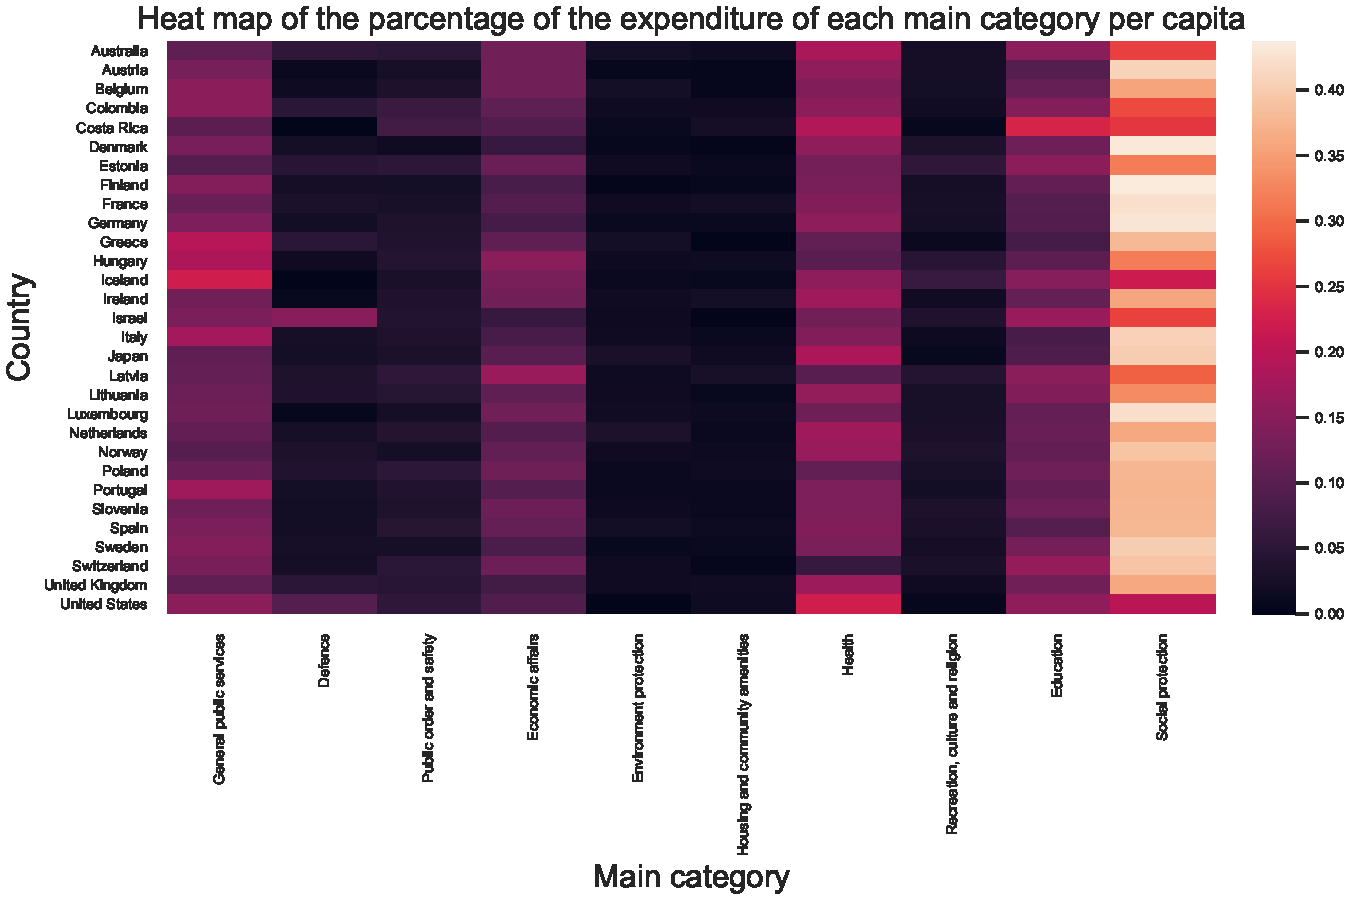
\includegraphics[width=0.85\linewidth]{figs/Heatmap_percentage.pdf}
\caption{Heatmap of average expenditure in each of the main COFOG categories for all countries in the dataset.}
\label{fig:scatter}
\end{figure}

To establish that government expenditure and happiness scores are in fact connected, we look at a scatter plot of total expenditure and happiness score in Figure \ref{fig:scatter}. Aside from a few outliers, we see a strong positive correlation, which motivated building a model.

\begin{figure}[h]
\centering
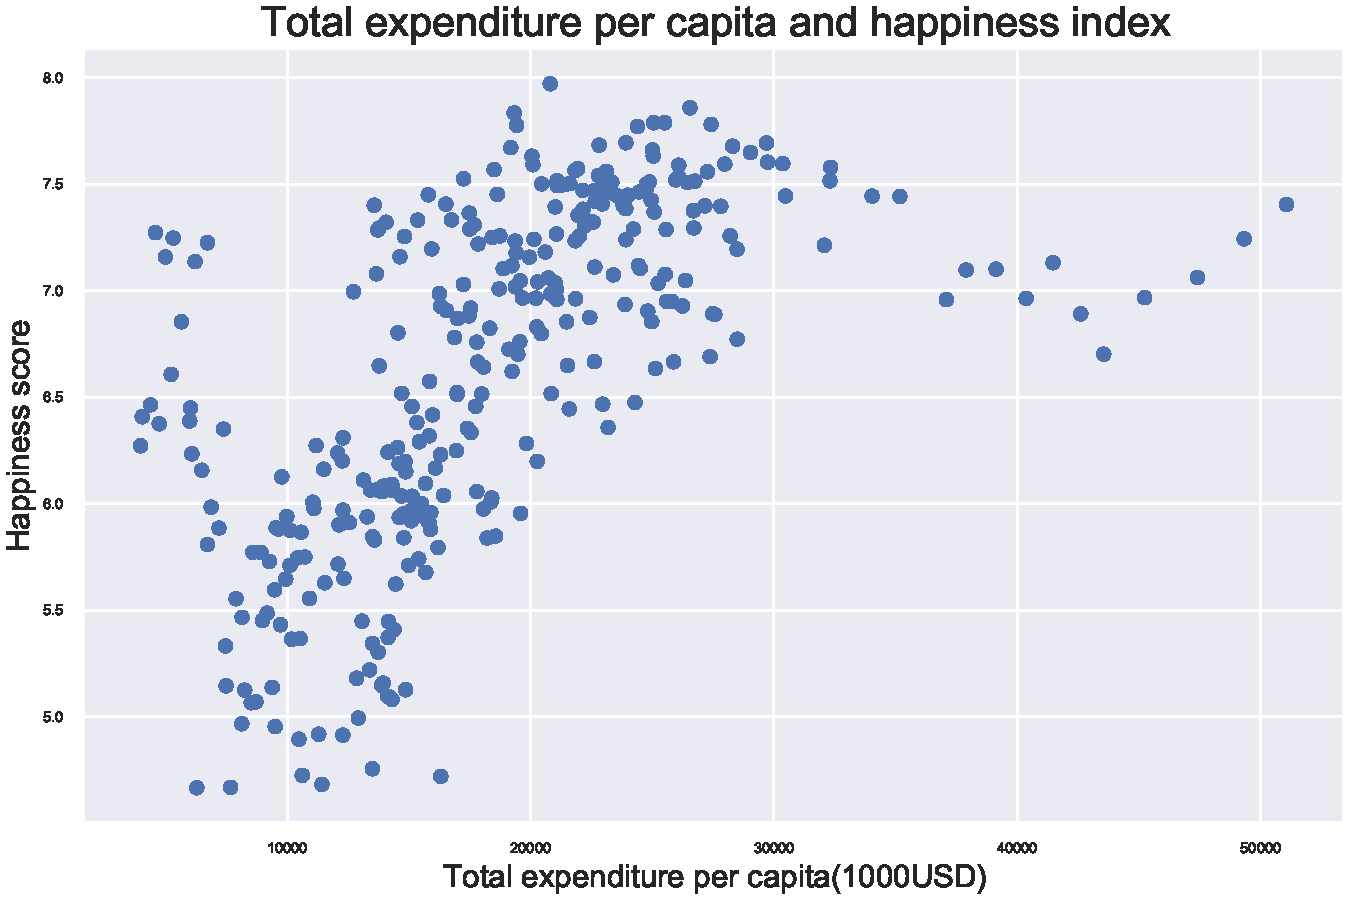
\includegraphics[width=0.5\linewidth]{figs/original_scatter_plot.pdf}
\caption{Scatter plot of total expenditure per capita crossed with happiness scores}
\label{fig:heatmap}
\end{figure}

\section{Methods}
We split the dataset into train and test sets in 80:20 ratio, giving us 66 samples in the test set and 261 samples in the train set. We train an unregularized linear regression, ridge regression and a feed-forward neural network \cite{neuralnetworks}, with hyperparameter grid as follows:

\begin{description}
   \item [Linear regression] Degree of polynomial in range 1 to 6.
   \item [Ridge regression] Degree of polynomial in range 1 to 6, regularization weight in range 0.1 to 10.
   \item [Feed-forward neural network] Solver LBFGS \cite{lbfgs}, Hidden layer sizes (5, 10, 15, 20, 25), Number of hidden layers (1, 2), Maximum iterations 2000
\end{description}

To evaluate the best model, we use 5-fold cross-validation and average the \(R^2\) coefficients \cite{r2}.
\subsection{Features}
We use only values of expenditure in all functions as features. However, as we have only 327 samples, we considered 69 features for all expenditure subcategories might increase the capacity of the model too much with not enough data to fit it. Therefore, we consider in addition a version of the dataset with expenditure in only the top level COFOG categories as features.

In addition, we also consider 2 cases of units of the expenditure value - As a percentage of total expenditure and as 1000USD per capita. We do this to gain insight into how much does the size of the expenditure budget in different countries matter in the happiness score.

\section{Results}
The results of best models for each version of the dataset are summarized in Table \ref{tab:results}.

\begin{table}[h]
\centering
\begin{tabular}{|l|l|l|c|} \toprule
Categories & Unit & Model & \(R^2\) score \\ \midrule
Parent & Percent & Linear P=3 & 0.34491 \\ \cline{3-4}
&  & Ridge P=6 A=0.1 & 0.20214 \\ \cline{3-4}
&  & Neural A=1e-5 S=25 L=2 & 0.56011 \\ \cline{2-4}
& USD per cpt & Linear P=2 & 0.09892 \\ \cline{3-4}
&  & Ridge P=2 A=10 & 0.59707 \\ \cline{3-4}
&  & Neural A=1e-05 S=10 L=1 & -1.0740 \\ \cline{1-4}
Subcategory & Percent & Linear P=1 & 0.83180 \\ \cline{3-4}
&  & Ridge P=2 A=0.1& 0.54760 \\ \cline{3-4}
&  & Neural A=1e-5 S=25 L=1 & 0.86060 \\ \cline{2-4}
& USD per cpt & Linear  P=1 & 0.05527 \\ \cline{3-4}
&  & Ridge P=1 A=4.6 & 0.81911 \\ \cline{3-4}
&  & Neural A=1e-5 S=5 L=1 & 0.33712 \\ \bottomrule
\end{tabular}
\caption{Results for each model with best found hyperparameters. Hyperparameter shortcuts - P - polynomial degree, A - alpha, S - neural layer size, L - number of hidden layers}
\label{tab:results}
\end{table}


We can see that best results are achieved on the dataset including all subcategories and with expenditure values as percentages. This is surprising, as it indicates how the government budget is divided is more important than the size of the budget. Best results were achieved by the neural model with score 0.860, but it is shockingly closely followed by a simple linear model without any polynomial features with a score of 0.831. Results of evaluating these 2 models on the test set can be seen in Table \ref{testres}. Given the interpretability advantages of linear models, we will inspect this model to gain insight into the importance of individual features. 

\begin{table}[h]
\centering
\begin{tabular}{|l|c|c|} \toprule
Model & \(R^2\) & MSE \\ \midrule
Linear & 0.852 & 0.078 \\ \cline{1-3}
Neural & 0.816 & 0.097 \\ \cline{1-3}
\end{tabular}
\caption{Results of best models on test set}
\label{tab:testres}
\end{table}


We show 3 most positively predictive features , 3 most negatively predictive features and 3 least predictive features in Table \ref{pospredfts}. More can be found in our GitHub repository.

\begin{table}[h]
\centering
\begin{tabular}{|l|l|c|c|} \toprule
Category & Parent category & Weight & Happiness per 1\% investment  \\ \midrule
R\&D Health & Health & 78.120285 & 0.781203 \\
Foreign economic aid & General public services & 49.168607 & 0.491686 \\
Communication & Economic affairs & 45.218878 & 0.452189 \\
R\&D Social protection & Social protection & -391.729622 & -3.917296 \\
Street lighting & Housing \& community & -242.087150 & -2.420871 \\
R\&D Housing \& community & Housing \& community& -170.847295 & -1.708473 \\
Old age & Social protection & 0.038013 & 0.000380 \\
Pre-primary and primary education & Education & 0.245861 & 0.002459 \\
Public order and safety n.e.c & Public order and safety & -0.365145 & -0.003651 \\ \bottomrule
\end{tabular}
\caption{Top 3 positively predictive features, Top 3 negatively predictive features, Top 3 least predictive features}
\label{pospredfts}
\end{table}

\section{Discussion}
We have achieved a surprisingly low prediction errors even with a simple linear model. However, one of the biggest flaws in the analysis was the lack of data.
It is possible more complex models could be used with more data, perhaps leading to better results. It should also be noted that our results do not imply increase in expenditure in a positively correlated areas would be a cause for increased happiness. Our model is trained to predict happiness in the same year the expenditure happened, where it's unlikely to have had a major effect on the population yet. As an example, it is unlikely that funding in the most negatively correlated feature, R\&D Social protection, is making the populace extremely angry. Rather, it is a topic for further research to explore confounding factors underlying happiness and the decision of governments to fund certain functions. It is also for this reason we have decided not to attempt to find the ideal budget allocation that would maximize predicted happiness scores. Such results would be possibly misleading.


\bibliographystyle{plain}
\bibliography{refs}

\end{document}
